\documentclass[conference]{IEEEtran}

\usepackage[utf8]{inputenc}
\usepackage{hyperref}
\usepackage{titlesec}
\usepackage{graphicx}
\usepackage{mathtools}
\usepackage{amsfonts}
\usepackage{amssymb}
\usepackage{amsmath}
\usepackage{cleveref}
\usepackage{listings}
\usepackage{color}
\usepackage{booktabs}
\usepackage{multirow}
\usepackage{subfigure}
\usepackage{float}
 
\definecolor{codegreen}{rgb}{0,0.6,0}
\definecolor{codegray}{rgb}{0.5,0.5,0.5}
\definecolor{codepurple}{rgb}{0.58,0,0.82}
\definecolor{backcolour}{rgb}{0.95,0.95,0.92}
 
\lstdefinestyle{mystyle}{
    backgroundcolor=\color{backcolour},   
    commentstyle=\color{codegreen},
    keywordstyle=\color{blue},
    numberstyle=\tiny\color{codegray},
    stringstyle=\color{codepurple},
    basicstyle=\footnotesize,
    breakatwhitespace=false,         
    breaklines=true,                 
    captionpos=b,                    
    keepspaces=true,                 
    numbers=left,                    
    numbersep=5pt,                  
    showspaces=false,                
    showstringspaces=false,
    showtabs=false,                  
    tabsize=4
}
 
\lstset{style=mystyle}

\inputencoding{utf8}
\titleformat*{\section}{\large\bfseries}
\newcommand\tab[1][1cm]{\hspace*{#1}}
\renewcommand{\lstlistingname}{Algoritmo}% Listing -> Algoritmo
\renewcommand{\figurename}{Figura}
\renewcommand{\tablename}{Tabla}

\begin{document}

\title{Tabu Search Applied in the Optimization in Static Regime for the Location of Police Resources in Asuncion, Paraguay}

\author{\IEEEauthorblockN{Luis Alberto Alvarez Penayo}
\IEEEauthorblockA{\textit{Facultad Politécnica} \\
\textit{Universidad Nacional de Asunción}\\
San Lorenzo, Paraguay \\
\href{mailto:lalvarez.pol@gmail.com}{lalvarez.pol@gmail.com}}
\and
\IEEEauthorblockN{Marco Antonio Alvarez Penayo}
\IEEEauthorblockA{\textit{Facultad Politécnica} \\
\textit{Universidad Nacional de Asunción}\\
San Lorenzo, Paraguay \\
\href{mailto:marcoalvarez@outlook.com}{marcoalvarez@outlook.com}}
\and
\IEEEauthorblockN{Diego Pedro Pinto Roa}
\IEEEauthorblockA{\textit{Facultad Politécnica} \\
\textit{Universidad Nacional de Asunción}\\
San Lorenzo, Paraguay \\
\href{mailto:dpinto@pol.una.py}{dpinto@pol.una.py}}
}

\maketitle

\begin{abstract}
The response time to 911 emergency calls is a very common problem in almost all developing countries. The optimization of this time is essential in achieving the goal of capturing the perpetrator of the crime and thus increasing the confidence towards the police force from the public. This paper seeks to optimize the response time in the displacement of police resources once they have been assigned to the incident, through a better geographic positioning taking into account the history of incidents that occurred over a period of time. For that a mathematical model and a tabu search algorithm are proposed. %As a basis for the tests, the city of Asunción and a history of two years of incidents were taken into account. The results showed that by strategically positioning the police resources, the response time to a emergency call could be considerably reduced.\\
%El tiempo de respuesta a una llamada de auxilio en las llamadas al 911 es un problema muy común en casi todos los países en desarrollo. En este trabajo se busca optimizar el tiempo de respuesta en el desplazamiento de los recursos policiales una vez que hayan sido asignados al incidente, mediante un mejor posicionamiento geográfico tomando en cuenta el historial de incidentes ocurridos en un lapso de tiempo. Como base para las pruebas se tomaron en cuenta la ciudad de Asunción y un historial de dos años de incidentes. Los resultados demostraron que mediante el posicionamiento estratégico de los recursos policiales se podría reducir considerablemente el tiempo de respuesta a una llamada de auxilio así como también reducir costos operativos al Estado paraguayo.\\
\end{abstract}
\begin{IEEEkeywords}
Computer aided analysis, Metasearch, Process planning, Operations research, Government.
\end{IEEEkeywords}

\section{Introdución}
La seguridad ciudadana constituye uno de los principales problemas sociales de varios países de América Latina, cuyos ciudadanos están profundamente preocupados por el fuerte incremento en la tasa de criminalidad, se sienten cada vez más inseguros en sus personas y bienes, y expresan su insatisfacción con respecto a la respuesta estatal ante el fenómeno delictivo\cite{rico2002seguridad}.\\
El fenómeno delictivo es un tema complejo, y muchas veces parece que cualquier acción que se realice para prevenirlo o controlarlo resulta insuficiente. Para esto es fundamental desarrollar diagnósticos de calidad basados en indicadores válidos y confiables\cite{ensc2014}.\\
En Paraguay, la Policia Nacional cuenta con jefaturas zonales y departamentales. Las jefaturas departamentales se subdividen en comisarías. La ciudad de Asunción cuenta con veinticuatro (24) comisarias; éstas tienen a su cargo cuatro o cinco cuadrantes, en los que operan un vehículo con dos o tres policías y a su vez, cada cuadrante se subdivide en sectores\cite{ensc2014}. \\
En fecha del 18 de octubre de 2012, fue sancionada la Ley que crea el Sistema Nacional de Emergencias denominado 911, para la atención de comunicaciones de emergencias. El sistema 911 funciona en un moderno centro de comando y recibe aproximadamente 7 mil llamadas diarias. Para tal tarea, un total de 45 efectivos policiales trabajan en tres turnos en el centro de comando y dirigen la labor de 120 patrulleros en Asunción y 400 en el Gran Asunción -preliminarmente administrados por el 911 y ahora adscritos a las comisarías-, de los cuales solo 114 tienen GPS en la actualidad. Se calcula que cada vehículo recorre diariamente entre 100 y 150 kilómetros\cite{ensc2014}.\\
Las llamadas dirijidas al 911 pasan por 4 etapas de tiempos [\cref{fig:time1}], que están definidas como (1) recepción, (2) procesamiento, (3) asignación del recurso policial encargado y (4) desplazamiento del recurso asignado.
\begin{figure}[!h]
    \centering
    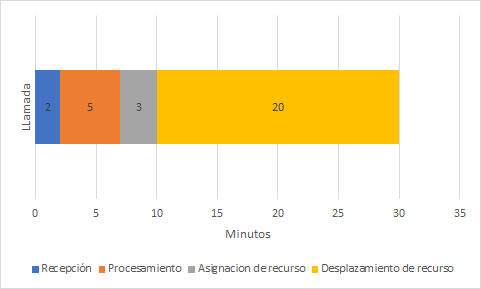
\includegraphics[width=100mm,scale=0.5]{images/tiempo_llamadas.png}
    \caption{Tiempo de vida promedio por llamada.}
    \label{fig:time1}
\end{figure}
\\A partir de lo citado anteriormente, se tomó como referencia el trabajo de [N. MENDES and A. SANTOS]\cite{mendesd} para obtener posiciones óptimas en la ubicación de los recursos policiales utilizando el procedimiento metaheurístico de la búsqueda Tabú. A fin de obtener valores más precisos fueron necesarios aplicar modificaciones al trabajo referenciado, los que serán detallados en las siguientes secciones.\\
Este trabajo, se enfoca en la optimización de la etapa 4 (desplazamiento del recurso) de las llamadas [\cref{fig:time1}], de tal forma a reducir al mínimo posible el tiempo transcurrido desde el inicio de la llamada hasta la asistencia del recurso policial, mediante la utilización del histórico de datos delictivos con georeferencias.

\section{Descripción del Problema}
En Paraguay, la Policía Nacional cuenta con jefaturas zonales y departamentales. Las jefaturas departamentales se subdividen en comisarías. La ciudad de Asunción cuenta con veinticuatro (24) comisarias; éstas tienen a su cargo cuatro o cinco cuadrantes, en los que operan uno o más vehículos con dos o tres policías y a su vez, cada cuadrante se subdivide en sectores. 

El Centro de Atención de Emergencias del Sistema 911 actualmente funciona como un simple call center de recepción de llamadas, en donde se registran los datos preliminares del incidente y este luego es despachado a la  institución integrante del Sistema \cite{ley4739} dependiendo del tipo de incidente denunciado. En los incidentes concernientes a la seguridad ciudadana actúa la Policía Nacional que cuenta, en las oficinas del 911, con oficiales encargados de gestionar la asignación de los recursos Policiales en coordinación con las comisarias responsables de cubrir los cuadrantes y sectores donde ocurrió el incidente, así también se debe dar seguimiento y registro de las novedades del incidente, hasta su cierre.

Son varios los problemas que actualmente enfrenta el Sistema 911 que impiden lograr un óptimo desempeño, tales como:
\begin{itemize}
\item Los recursos policiales que deben acudir a un llamado no siempre se encuentran disponibles, debido a que al ser dependientes de las comisarias cumplen también otras funciones de seguridad y no exclusivamente atención de emergencias, por tanto podrían inclusive darse casos donde al no disponer una comisaria de recursos para cubrir su cuadrante, esta deba solicitar apoyo a algún recurso disponible de alguna comisaria cercana.
\item Incumplimiento del requisito mínimo de infraestructura, donde las telefonías tienen la obligación de facilitar la localización de la llamada a través de un sistema automático de identificación. Sin los datos exactos de ubicación del llamante se dificulta la tarea del operador de identificar exactamente el lugar del hecho, incurriendo en imprecisiones en las indicaciones.
\item Los patrullajes realizados por los recursos para la mitigación de los hechos de inseguridad son realizados de forma aleatoria sin considerar ninguna base de información ni siguiendo algún procedimiento establecido para el efecto que permita medir los resultados y efectividad del procedimiento realizado. 
\end{itemize}

Estos y otros problemas inciden directamente en el tiempo de desplazamiento del recurso ante un incidente, siendo este tiempo mayor al 60\% del tiempo total requerido para atender efectivamente un llamado.

Por ello este trabajo se centra en aplicar la Búsqueda Tabú como metodología científica que permita reducir el tiempo de desplazamiento. A su vez, nos permite obtener una optimización en cuanto a la asignación de los recursos disponibles considerando datos estadísticos que nos arrojan las zonas críticas a ser cubiertas. Como resultados del algoritmo podemos obtener una o varias combinaciones de posibilidades de cobertura que garanticen un tiempo de respuesta mínimo así como también un mayor grado de cobertura global.

\section{Metodología Actual}
El método actual utilizado para el posicionamiento de los recursos policiales está determinado por lo que dicte el comisario de turno de la comisaría a la que corresponde el recurso. El caso habitual es que un recurso es ubicado aleatoriamente dentro del cuadrante que corresponde a su comisaría realizando un patrullaje por sus alrededores.

Al estar los recursos bajo la dependencia de las comisarías, éstas no siempre se encuentran disponibles para atender un llamado de emergencia ya que podrían estar siendo utilizadas para tareas competentes a las comisarias como ser traslados de reclusos o allanamiento de algún lugar.

El manejo de este tipo de situaciones donde no se encuentra disponible el recurso dentro de su cuadrante se solventa mediante el pedido de un recurso a una comisaría vecina, que se encuentre lo más cercano al lugar donde ocurrió el llamado de emergencia.

\section{Modelado}
El modelado tratado más abajo está basado en el trabajo presentado en \cite{7359471}.

El mapa fue modelado como un grafo conexo $G = (V, E)$ ponderado y direccionado, de forma que dos vértices (intersecciones de tramos) $v, w \in V$ que son adyacentes siempre están unidos por dos aristas $e_{1}, e_{2} \in E$ (tramos), una yendo de $v$ hacia $w$ y la otra realizando el sentido contrario. Cada tramo $r \in E$ posee un nivel de violencia $l_{r}$ y una longitud $d_{r}$ (distancia entre las intersecciones limitantes)\cite{van2010introduction}. A partir de la longitud es calculado el tiempo empleado por cada tipo de unidad en recorrerlo. Si los tramos son de sentido único, se considera un incremento del 50\% en el tiempo necesario para recorrerlo en el sentido contrario para todos los vehículos motorizados, buscando simular la dificultad de esos recursos para recorrer el tramo. Además, algunas aristas representan tramos que no pueden ser transitadas mediante el uso de vehículos motorizados. Para modelarlas, fue considerado que el tiempo necesario para recorrerlas es $-1$ (menos uno). Un oficial recorriendo a pie no posee tramos con tiempo $-1$.

Además, se define un conjunto $U$ de recursos policiales disponibles. Cada recurso posee un tipo $i \in Q$ (tal que $Q$ es el conjunto de todos los tipos de recursos), que define las condiciones de movilidad de estas. Para cada uno de estos tipos es definido también una cantidad $U_{i}$ de recursos disponibles.

Para decir que un recurso ubicado en una intersección $v$ elije un tramo $r$, es definido un tiempo límite $T_{max}$ para salir de $v$ y llegar a una de las intersecciones de $r$, considerando las correcciones de tiempos tales como las tratadas anteriormente.

El nivel de violencia asociado a cada tramo $l_{r}$ es obtenido mediante el cálculo de la distribución de Poisson\cite{moreno1995manual} utilizando el histórico de los delitos. Como los delitos se encuentran asociados a las intersecciones, para obtener la cantidad de delitos por tramo se considera el promedio de los delitos en cada extremo.

Para la construcción del modelo son utilizadas las siguientes variables de decisión:

$x_{ij}$: Variable que indica la cantidad de recursos del tipo $i$ ubicadas en el vértice $j$.

$a_{r}$: Variable binaria igual a $1$ si el tramo $r$ es cubierto por algún recurso policial dentro del tiempo $T_{max}$, y $0$ en caso contrario.

$a'_{r}$: Similar a la anterior, pero con tiempo $2T_{max}$.

$p_{rji}$: Variable binaria igual a $1$ si un recurso de tipo $i$ ubicado en $j$ logra cubrir el tramo $r$ en tiempo $T_{max}$, y $0$ en caso contrario.

$p'_{rji}$: Similar a la anterior, pero con tiempo $2T_{max}$.

$N$: Variable que indica la cantidad de tramos no alcanzables en un tiempo $2T_{max}$.

$W$: Constante que almacena el mayor valor posible que toma la función objetivo sin penalización.

Dicho modelo es mostrado a continuación:
\begin{alignat}{2}
    maxZ\label{eq:optimization-funtion}
    &= \sum_{r \in E} l_{r}a_{r} - P(N)\\
    P(N)\label{eq:penalization}
    &= NW\\
    \sum_{j \in V} x_{ij}\label{eq:total-resource}
    &\leq U_{i}, 
    &&\tab\forall i \in Q\\
    a_{r}\label{eq:p-resource}
    &\leq \sum_{i \in Q}\sum_{j \in V} p_{rij}x_{ij}, 
    &&\tab\forall r \in E\\
    a'_{r}\label{eq:pprime-resource}
    &\leq \sum_{i \in Q}\sum_{j \in V} p'_{rij}x_{ij}, 
    &&\tab\forall r \in E\\
    \sum_{r \in E} a'_{r}\label{eq:all-edges}
    &= |E|\\
    x_{ij}\label{eq:xvariable}
    &\in \mathbb{Z^{+}}, 
    &&\tab\forall i \in U, \quad j \in V\\
    a_{r}, a'_{r}\label{eq:binaries} 
    &\in \{0,1\}, 
    &&\tab\forall r \in E\\
    N, W\label{eq:penal-variables} 
    &\in \mathbb{Z^{+}}
\end{alignat}

En la función objetivo (\ref{eq:optimization-funtion}) se buscar maximizar el valor obtenido de la sumatoria del nivel de violencia de todos los tramos que son cubiertos (alcanzados en tiempo $T_{max}$) por al menos un recurso policial, disminuyendo el valor por una función de penalización. La función de penalización (\ref{eq:penalization}) está definida como la cantidad de tramos no cubiertos por algún recurso multiplicado por el máximo valor posible de la función objetivo. En la restricción (\ref{eq:total-resource}) es definido el número máximo de recursos de cada tipo que puede ser ubicado. Para la restricción (\ref{eq:p-resource}) el valor de la variable que define si un tramo es cubierto y definido a través de la verificación si existe algún recurso ubicado en un punto suficientemente próximo de este tramo. En (\ref{eq:pprime-resource}) es hecha básicamente la misma cosa, pero la distancia considerada es el doble. La restricción (\ref{eq:all-edges}), garantiza que todo tramo debe ser alcanzado por al menos un recurso policial en un tiempo máximo $2T_{max}$. Por ultimo, las restricciones (\ref{eq:xvariable}) y (\ref{eq:penal-variables}) indican la integridad de las variables $x_{ij}$, $N$ y $W$, y la restricción (\ref{eq:binaries}) indica que las variables $a_{r}$ y $a'_{r}$ son binarias.

\subsection{Búsqueda Tabú}
La Búsqueda Tabú es una meta-heurística basada en búsqueda local en donde algunas alteraciones en la cadena de respuesta son prohibidas de realizarse por un cierto número de iteraciones\cite{glover1989tabu}. Estas alteraciones prohibidas permanecen almacenadas en una estructura llamada lista tabú, de donde viene el nombre del algoritmo.

Como parámetro de entrada el algoritmo requiere de una solución inicial, para obtener esta solución fue necesario calcular los valores de cobertura que definimos a continuación como:
\begin{alignat}{2}
    C_{ri}\label{eq:cobertura}
    &= \sum_{r \in E} l_{r}a_{r} 
    &&\tab\forall r \in E, \forall i \in Q
\end{alignat}

En base a (\ref{eq:cobertura}) decimos que, para cada arista del grafo y por cada tipo de recurso es calculado su área de cobertura a través de la suma de los niveles de violencia sin tener en cuenta si el tramo fue cubierto previamente por otro recurso.

Una vez que se obtienen todos los valores de cobertura, se eligen aleatoriamente los vértices donde irán ubicados cada tipo de recursos (atendiendo que un recurso motorizado tenga al menos un tramo por donde movilizarse considerando la restricción de accesos).

\lstinputlisting[language=Ruby,caption={Pseudo código de Búsqueda Tabú},label=alg:tabusearch]{tabu.code}

La búsqueda fue definida como muestra el algoritmo \ref{alg:tabusearch}, primeramente se obtiene la solución inicial (línea 1) luego se inicializan las variables básicas (líneas 2 al 4). Ya en la búsqueda local, el proceso itera un máximo de veces definido por $4|U|$ (línea 5), donde un recurso es seleccionado aleatoriamente (línea 6) y se evalúa entre todos los vecinos de ese recurso cual de ellos es el que mejor ubicado, teniendo en cuenta la función objetivo así como también que no pertenezca a un vecino tabú (líneas 9 al 16). Luego de seleccionar el mejor vecino se comprueba si éste contribuye a mejorar la solución global (líneas 18 al 21). Por último, a cada $|U|$ iteraciones se realiza un proceso de intensificación de forma a generar soluciones más viables. Este proceso se rige de acuerdo a los pasos: (1) escoger un recurso sin restricción de acceso, (2) se coloca un recurso en un vértice de alguna arista no cubierta en tiempo $2T_{max}$, (3) la unidad con la mayor intersección en área de cobertura con la unidad reubicada (considerando la nueva posición) es llevada a la posición original de la unidad reubicada, (4) se hace una búsqueda local en 15 de los nodos cubiertos en tiempo $2T_{max}$ por la unidad reubicada en su nueva posición, para hacer un ajuste más fino de la nueva posición de esa unidad.

\section{Experimentos y Resultados}
Para la conformación del mapa de pruebas se tomó en cuenta la zona geográfica más confluida de la ciudad de Asunción, la zona céntrica, donde se concentra el ámbito empresarial, y que además posee lugares turísticos como ser el Palacio de Gobierno, la Catedral Metropolitana, la Avda. Costanera, y el casco histórico. Esta región de pruebas conforma un un grafo con 2306 vértices y 6376 aristas.

Dentro del área de trabajo definida se pudo denotar que el mismo se encontraba dentro de los cuadrantes de 6 comisarías del área metropolitana, por lo que primeramente se calculó el porcentaje de área que correspondía a cada cuadrante, luego, en base a este porcentaje fue calculado también la cantidad recursos por tipos a utilizar para las pruebas (redondeando el valor obtenido hacia el entero inferior), siendo el promedio de recursos por tipo con el que cuenta cada comisaría de 4 patrulleras, 2 motocicletas, y 3 oficiales a pie. Así, el total de recursos utilizados fue de 12 patrulleras, 5 motocicletas, y 8 oficiales. En la tabla \ref{table:calculo-recursos}, se muestran las distribuciones de recursos por cada comisaria en base a lo mencionado anteriormente.

Fueron utilizados tiempos de $T_{max}$ igual a 3 minutos y $2T_{max}$ de 6 minutos para la comparación de la metodología actual con la solución propuesta.

Para emular la metodología actual del posicionamiento de los recursos, fueron ubicados aleatoriamente cada uno de ellos dentro del cuadrante correspondiente a sus comisarias. Y para el caso de la Búsqueda Tabú como no se circunscriben las ubicaciones de los recursos dentro de la limitante de los cuadrantes, estos se ubican aleatoriamente dentro del área considerada, con la única restricción de cantidad de recursos y su cobertura intrínseca por tipo, previamente calculadas.

La presentación gráfica de los resultados cuenta con el mapa base de pruebas donde se pueden visualizar todos los tramos de la zona geográfica escogida, y un mapa de calor delictivo donde los puntos en rojo representan los lugares donde se encuentran un mayor número de tramos con niveles de violencia elevado.

En la figura \ref{fig:mapas-cobertura}, se observan con estrellas los recursos ubicados en los diferentes puntos del mapa, los trazos en verde representan los tramos que fueron cubiertos por los recursos, mientras que los trazos en negro los no cubiertos en el tiempo $2T_{max}$ por algún recurso.

El caso particular para \ref{fig:estocastico}, la distribución de los recursos no sigue ningún patrón determinado, simplemente se ubican aleatoriamente.

La tabla \ref{table:resultados-estocastico}, nos indica el valor de cobertura obtenido por cada uno de los recursos y el total de las coberturas, tanto por recurso como así en el área considerada.

En la figura \ref{fig:tabusearch}, observamos las nuevas ubicaciones basadas en la Búsqueda Tabú. Se puede observar a simple vista que la cantidad de tramos en negro es casi inexistente, indicando una cobertura casi total del área. Además de esto, también se observa cómo los recursos de mayor movilidad, los motorizados, se ubican en mayor cantidad hacia las zonas de más alto nivel de violencia, mostrado por el mapa de calor.

En la tabla \ref{table:resultados-tabu}, se denotan los valores de cobertura por cada uno de los recursos ubicados, en la cual se puede observar la particularidad de que los recursos a pie que tienen valores muy bajos e incluso cero, confirmando lo dicho anteriormente de la prioridad dada a los recursos motorizados, demostrando que la solución propuesta posee una capacidad de optimizar la ubicación priorizando la cobertura de cada tipo.

Tras las pruebas realizadas se pudo constatar que, para el área de trabajo definido los recursos no fueron suficientes para cubrir la totalidad de los tramos. Siendo el problema que la alta cantidad de tramos de accesos restrictivos superaba en gran medida la limitada cantidad de recursos a pie con los que se disponía.

\begin{table}[]
\centering
\caption{Recursos a ser utilizados, por tipo, en el área considerada.}
\label{table:calculo-recursos}
\begin{tabular}{@{}ccccccc@{}}
\toprule
\multirow{2}{*}{\textbf{Comisaría}} & \multirow{2}{*}{\textbf{Cobertura}} & \textbf{Patrulleras}                    & \multicolumn{1}{l}{} & \textbf{Motos}                          & \multicolumn{1}{l}{} & \textbf{Oficiales}                      \\ \cmidrule(lr){3-3} \cmidrule(lr){5-5} \cmidrule(l){7-7} 
                                    &                                     & \multicolumn{1}{l}{\textbf{(Prom. 4)}} & \multicolumn{1}{l}{} & \multicolumn{1}{l}{\textbf{(Prom. 2)}} & \multicolumn{1}{l}{} & \multicolumn{1}{l}{\textbf{(Prom. 3)}} \\ \midrule
\textbf{18va}                       & 33\%                                & 1                                       &                      & 0                                       &                      & 1                                       \\
\textbf{4ta}                        & 50\%                                & 2                                       &                      & 1                                       &                      & 1                                       \\
\textbf{3ra}                        & 55\%                                & 2                                       &                      & 1                                       &                      & 1                                       \\
\textbf{5ta}                        & 100\%                               & 4                                       &                      & 2                                       &                      & 3                                       \\
\textbf{9na}                        & 33\%                                & 1                                       &                      & 0                                       &                      & 1                                       \\
\textbf{21ra}                       & 50\%                                & 2                                       &                      & 1                                       &                      & 1                                       \\ \midrule
\multicolumn{2}{c}{\textbf{Total Recursos}}                               & 12                                      &                      & 5                                       &                      & 8                                       \\
\bottomrule
\end{tabular}
\end{table}
\begin{table}
\centering
\caption{Niveles de violencia cubiertos por tipo de recurso - Método aleatorio}
\label{table:resultados-estocastico}
\begin{tabular}{crrrr}
\toprule
\textbf{Recurso} & \multicolumn{1}{c}{\textbf{Patrullera}} & \multicolumn{1}{c}{\textbf{Moto}} & \multicolumn{1}{c}{\textbf{Oficial}} & \multicolumn{1}{c}{\textbf{Total}} \\ \hline
\textbf{1}       & 897.23                                  & 447.21                            & 0.00                                 & -                                  \\
\textbf{2}       & 381.24                                  & 979.29                            & 3.66                                 & -                                  \\
\textbf{3}       & 485.88                                  & 567.57                            & 0.00                                 & -                                  \\
\textbf{4}       & 634.22                                  & 356.39                            & 17.81                                & -                                  \\
\textbf{5}       & 278.02                                  & 234.16                            & 84.99                                & -                                  \\
\textbf{6}       & 889.30                                  & -                                 & 61.35                                & -                                  \\
\textbf{7}       & 3.88                                    & -                                 & 30.93                                & -                                  \\
\textbf{8}       & 109.14                                  & -                                 & 59.18                                & -                                  \\
\textbf{9}       & 179.11                                  & -                                 & -                                    & -                                  \\
\textbf{10}      & 287.53                                  & -                                 & -                                    & -                                  \\
\textbf{11}      & 328.30                                  & -                                 & -                                    & -                                  \\
\textbf{12}      & 229.26                                  & -                                 & -                                    & -                                  \\ \hline
\textbf{Total}   & \textbf{4703.11}                        & \textbf{2584.64}                  & \textbf{257.92}                      & \textbf{7545.67}                   \\
\bottomrule
\end{tabular}
\end{table}
\begin{table}
\centering
\caption{Niveles de violencia cubiertos por tipo de recurso - Búsqueda Tabú}
\label{table:resultados-tabu}
\begin{tabular}{crrrr}
\toprule
\textbf{Recurso} & \multicolumn{1}{c}{\textbf{Patrullera}} & \multicolumn{1}{c}{\textbf{Moto}} & \multicolumn{1}{c}{\textbf{Oficial}} & \multicolumn{1}{c}{\textbf{Total}} \\ \hline
\textbf{1}       & 601.93                                  & 872.46                            & 64.30                                & -                                  \\
\textbf{2}       & 605.68                                  & 746.71                            & 0.00                                 & -                                  \\
\textbf{3}       & 793.57                                  & 383.24                            & 0.00                                 & -                                  \\
\textbf{4}       & 414.79                                  & 430.10                            & 0.00                                 & -                                  \\
\textbf{5}       & 90.33                                   & 693.38                            & 0.00                                 & -                                  \\
\textbf{6}       & 254.78                                  & -                                 & 57.79                                & -                                  \\
\textbf{7}       & 5.66                                    & -                                 & 0.01                                 & -                                  \\
\textbf{8}       & 324.92                                  & -                                 & 80.42                                & -                                  \\
\textbf{9}       & 927.03                                  & -                                 & -                                    & -                                  \\
\textbf{10}      & 672.29                                  & -                                 & -                                    & -                                  \\
\textbf{11}      & 1048.04                                 & -                                 & -                                    & -                                  \\
\textbf{12}      & 550.66                                  & -                                 & -                                    & -                                  \\ \hline
\textbf{Total}   & \textbf{6289.68}                        & \textbf{3125.90}                  & \textbf{202.52}                      & \textbf{9618.10}                   \\
\bottomrule
\end{tabular}
\end{table}
\begin{figure}
    \begin{center}
        \subfigure[Método Aleatorio]{\label{fig:estocastico}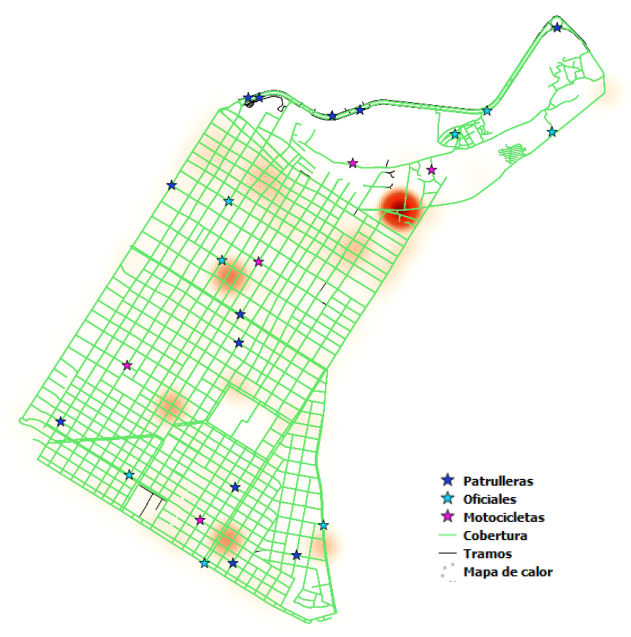
\includegraphics[width=90mm,scale=0.5]{images/estocastico_leyenda.png}}
        \subfigure[Búsqueda Tabú]{\label{fig:tabusearch}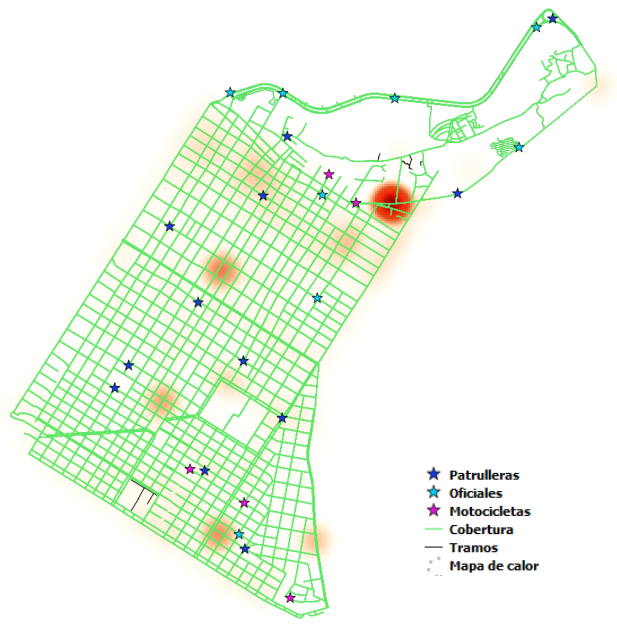
\includegraphics[width=90mm,scale=0.5]{images/tabusearch_leyenda.png}}
    \end{center}
    \caption{Mapas de cobertura por método}
    \label{fig:mapas-cobertura}
\end{figure}

\section{Evaluación de rendimiento}
Realizando una comparación entre ambas metodologías podemos observar, en la figura \ref{fig:comparativa}, que la búsqueda tabú prioriza a los recursos motorizados para la cobertura de las zonas con mayor nivel de violencia. Lo que a su vez produce un mayor valor en el nivel de violencia cubierto a nivel global.

Además de los resultados indicados anteriormente, cabe resaltar que el algoritmo aquí propuesto soluciona un problema multi-objetivo ya que además de priorizar la cobertura de las zonas con mayores niveles de violencia, intenta cubrir todas las aristas del grafo. Esto último, se puede apreciar fácilmente comparando las figuras \ref{fig:estocastico} y \ref{fig:tabusearch}.
\begin{figure}
    \centering
    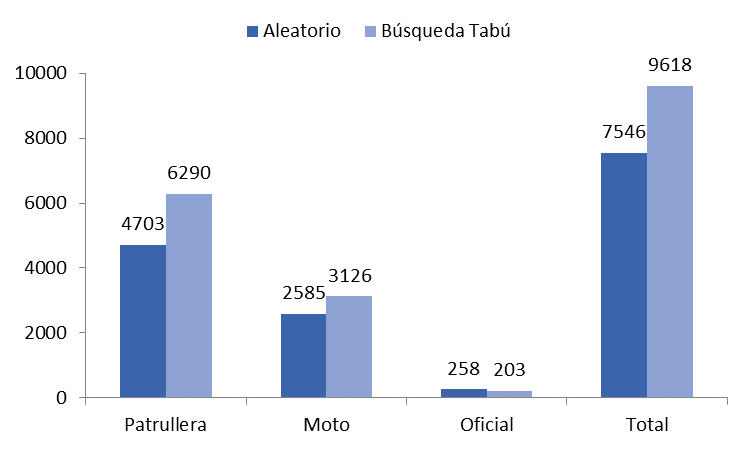
\includegraphics[width=88mm,scale=0.5]{images/comparativa.png}
    \caption{Niveles de violencia cubiertos por tipo de recurso en ambas metodologías.}
    \label{fig:comparativa}
\end{figure}

\section{Conclusión}
En este trabajo realizamos una implementación de la Búsqueda Tabú como propuesta de solución ante la problemática de ubicación óptima de recursos frente al modelo aleatorio utilizado actualmente.

En la evaluación de rendimiento, mostramos que la Búsqueda Tabú obtuvo en general mejores valores en cuanto a niveles de violencia cubiertos para los tipos de recursos patrulleras y motocicletas. En los casos de oficiales a pie no siempre se obtenían mejores valores, ésto debido a que el procedimiento de intensificación se encarga de optimizar el posicionamiento de recursos no motorizados en zonas donde no pueden ingresar vehículos.
Ambos modelos muestran un buen nivel de cobertura total para un tiempo máximo $T_{max}$ y $2T_{max}$.

A diferencia de la metodología actual, el trabajo propone que los recursos policiales (patrulleras, motocicletas y oficiales a pie) pertenezcan al Sistema Nacional de Emergencias 911 y no se encuentren adscritos a las comisarías, lo que facilita la libre ubicación de los mismos para optimizar las zonas críticas de cobertura.

Como trabajos futuros proponemos la evaluación de los delitos por franjas horarias de manera a tener diferentes posiciones de recursos acorde vaya transcurriendo las horas del día, ya que en algunas zonas el nivel de violencia aumenta o disminuye al movimiento de personas. Otro enfoque sería cambiar el algoritmo de la Búsqueda Tabú por el algoritmo Particle Swarm Optimization (PSO) o bien uno más reciente como el Bat-Algorithm.

\bibliographystyle{bibliography/IEEEtran}
\bibliography{bibliography/references}

\end{document}

